\chapter{Metodologia}
\label{chap:MatMet}

O Capítulo \ref{chap:FUNDA} apresentou alguns dos métodos encontrados na literatura para a representação computacional de formas a partir do seu contorno.  Em muitos casos, esses métodos apresentam parâmetros que requerem ajustes, sendo esse ajuste dependente da natureza da aplicação, ou seja,  das características da base de imagens e do propósito ao qual o sistema de reconhecimento se destina. A energia de dobramento multiescala, por exemplo, requer o ajuste do número e os valores dos fatores de escala utilizados na representação das formas. 

Esse capítulo apresenta um método robusto e versátil para o ajuste desses parâmetros para customizar esses descritores em aplicações de classificação supervisionada e não supervisionada.   
 

%Os descritores entropia multiescala, apresentado no Capítulo \ref{chap:FUNDA}, e a energia de dobramento multiescala requerem o ajuste dos seguintes parâmetros: o número e os valores dos fatores de escala utilizados na representação das formas. Esse capítulo apresenta um método robusto e versátil para o ajuste desses parâmetros para customizar esses descritores em aplicações de classificação supervisionada e não supervisionada.   
 

\section{Ajuste de parâmetros}
A metodologia para escolha de parâmetros do descritor segue o esquema da Figura \ref{fig:Avaliacao}. Essa metodologia melhora a representação do descritor utilizando métodos de otimização evolutivos para minimizar uma função custo que corresponde a mediana do erro absoluto da silhouette dos descritores ($MAD$). O que motivou a escolha dessa função custo é sua robustez a valores extremos \cite{Rousseeuw:1987:2}, sendo sua equação 

\begin{equation}
\label{eq:mad}
MAD = \operatorname{mediana}\big(|s_i - 1|_{i =1,\:2,\:\cdots,\:L}\big)\text{,}
\end{equation}

\begin{figure*}[ht]
\centering
\includegraphics[width=\textwidth,trim = 14mm 164mm 0mm 24mm,clip]{Final_Flux.pdf}
\caption{Proposta de uma metodologia para otimização evolucionária de um descritor multiescala de forma.} 
\label{fig:Avaliacao}
\end{figure*}

\noindent aonde $S = \{s_1,s_2,\cdots,s_L\}$ é o conjunto das \emph{silhouettes} calculadas para $L$ descritores de forma. Os operadores $|.|$  e {$mediana ( )$} retornam o valor absoluto e a mediana de um conjunto de valores, respectivamente.

A Silhouette \cite{Rousseeuw:1987} é uma medida de qualidade de agrupamentos que indica o grau de afinidade de uma amostra  a um agrupamento, levando em conta as distâncias médias entre-classes e intra-classes de um objeto $i$ atribuído a uma dada classe $A$. Logo, esta métrica é definida como 
\begin{equation}
s_i = \frac{b_i - a_i}{\max{(a_i,b_i)}} \in [-1,1],
\end{equation}

\noindent sendo $a_i$ a dissimilaridade média entre o objeto $i$ e os demais objetos pertencentes a mesma classe de $a_i$ e $b_i$ é a dissimilaridade média do objeto $i$ e a classe vizinha mais próxima de $i$, excluída sua própria classe. 

Essa métrica pode assumir valores no intervalo $[-1,1]$, sendo que valores negativos indicam que o grau de pertencimento de um objeto à classe que este fora atribuído é baixo. Já valores positivos indicam que o grau de pertencimento de um objeto à classe que este fora atribuído é alto. Um valor de silhouette próximo de zero indica que o objeto está na fronteira entre duas classes e que há, portanto, um grau de incerteza a respeito de qual classes este pertence.

Os valores da função objetivo $MAD$ assume valores no intervalo $[0,2]$. De forma análoga a silhouette, um valor igual a zero desta função indica que a estrutura dos clusters é perfeita, enquanto que valores próximos de $2$ indicam que a estrutura dos clusters é deficiente, com baixa similaridade entre os objetos de mesma classe ou alta similaridade entre os objetos de classes distintas.

A Figura  \ref{fig:Avaliacao} ilustra, em detalhes, como se dá o ajuste dos parâmetros do descritor multiescala dentro da metodologia proposta, bem como esta avalia a qualidade do descritor obtido com os parâmetros otimizados.  Primeiramente, é amostrado na base de folhas um sub-conjunto das formas para, em seguida, realizar o procedimento de otimização e encontrar o melhor conjunto de parâmetros de escala  $\boldsymbol{\sigma}_{otim} = (\sigma_1,\:\sigma_2,\:\cdots,\:\sigma_k)$ do descritor multiescala que minimize a função custo da Equação \ref{eq:mad}. Então, utilizando-se as escalas encontradas realiza-se, com o descritor multiescala, a extração de características de toda a base de folhas.

O desempenho do descritor, em termos de agrupamento das formas, é avaliado qualitativamente e quantitativamente. Na avaliação qualitativa dois algoritmos de visualização de dados são utilizados: o mapa auto-organizável de Kohonen \cite{Kohonen:2001} e o \textit{multidimensional scaling} \cite{cox:2000}. Esses algoritmos produzem projeções bi-dimensionais das descrições das formas da base de folhas, provendo uma representação gráfica que possibilita a análise da qualidade dos agrupamentos. Assim, consegue-se inferir o quão eficaz o descritor é em organizar espacialmente as formas. Já na avaliação quantitativa são analisadas métricas de avaliação obtidas em experimentos de classificação supervisionada (precisão e revocação), de recuperação de formas (bulls-eye) e a medida silhouette \cite{Rousseeuw:1987} média por classe. 

A silhouette média por classe avalia tanto a coesão como a separação das classes através da distância entre os vetores de características. Já as métricas de precisão e revocação são medidas clássicas na avaliação do desempenho de descritores em experimentos de classificação supervisionada. Na classificação supervisionada, os classificadores utilizados foram Naive Bayes (NB) \cite{Fukunaga:1990}, \emph{K}-vizinhos próximos (Knn, $K = 5$) \cite{Fukunaga:1990,Webb:2002},  o discriminante linear de Fisher (LDA) \cite{Webb:2002} e o discriminante quadrático (QDA) \cite{Fukunaga:1990}.  Antes da classificação com os classificadores NB e \emph{Knn} foi utilizado o discriminante linear de Fisher para transformar os dados \cite{Webb:2002}. Já para classificação com os classificadores LDA e QUA aplicou-se a análise das componentes principais para descorrelacionar os dados. Os experimentos realizados de recuperação de imagens pelo conteúdo visam avaliar o desempenho dos descritores de formas e das medidas de similaridade estudadas neste trabalho. As metodologias utilizadas nesses experimentos são as mesmas encontradas em diversos trabalhos de recuperação de formas da literatura.

Foram realizados experimentos em duas bases de imagens de formas binárias: a Kimia, de 99 formas, e a MPEG-7 CE-Shape-1 de 1400 formas. Ambas as bases estão apresentadas no Apêndice deste trabalho.

A  Figura \ref{fig:metodo_cbir} ilustra a metodologia dos experimentos de recuperação de formas.  Primeiramente realiza-se a extração de características das formas da base de imagens de formas binárias com o método de descrição sob avaliação. O mesmo processo de extração de características é aplicado a imagem de uma forma de consulta. Esse processo resulta numa base de dados com os vetores de características associados às formas utilizadas no experimento. 

Com a medida de similaridade avalia-se o grau de correspondência existente entre o vetor de características da forma de consulta e os vetores associados a cada uma das formas da base. Tem-se assim como resultado uma lista de imagens recuperadas em ordem decrescente de similaridade à forma de consulta. Todo esse processo é realizado repetidamente tomando-se cada forma da base de imagens como forma de consulta e recuperando-se as demais.

\begin{figure}[h!]
  \caption{\label{fig:metodo_cbir} Metodologia empregada para os experimentos de recuperação de formas pelo conteúdo.}
  \centering
  \includegraphics[width=0.55\textwidth]{Metodologia1.jpg}
\end{figure}

Na avaliação do desempenho dos experimentos duas medidas são utilizadas: o número total de acertos por posição recuperada e a medida Bull-eye.

A primeira medida consiste no número total de ocorrências de formas da mesma classe que a forma de consulta em cada posição recuperada.  Em diversos trabalhos de recuperação de formas pelo conteúdo o número total de acertos por posição recuperada é calculado para a base Kimia-99 \cite{Bernier:2003}. Tendo esta base 99 formas, igualmente distribuídas em 9 classes, são realizadas 99 recuperações das 11 formas mais similares à imagem de consulta. Como resultado espera-se obter um total de 99 formas recuperadas corretamente para cada posição recuperada.

A medida Bulls-eye também é utilizada na literatura para a comparação de diferentes métodos de recuperação de formas. Essa medida é calculada para a base MPEG-7 CE-Shape-1 da seguinte maneira: tomando-se cada forma dessa base de imagens como elemento de consulta, contabiliza-se o número de recuperações pertencentes a mesma classe da forma de consulta dentre as 40 primeiras posições recuperadas. Como resultado calcula-se a percentagem da quantidade máxima de recuperações corretas possíveis de se alcançar, sendo esta última quantidade $28000 = 1400\text{ formas} \times 20\text{ recuperações corretas poro forma}$. 


%A avaliação de similaridade entre formas a partir de medidas de divergência requer que as informações das assinaturas, abordadas na Seção \ref{sec:Assinatura} do Capítulo \ref{chap:contour}, sejam tratadas como variáveis aleatórias e que suas distribuições de probabilidade sejam estimadas. 

%A  Figura \ref{fig:metodo_distancia} ilustra como divergentes podem ser aplicados na avaliação da similaridade entre duas formas A e B. No método em questão, as distribuições de probabilidade de quatro assinaturas distintas dos contornos das formas são estimadas, através de histogramas, para em seguida se calcular as medidas de divergência. Uma medida de similaridade é então obtida  a partir da média ponderada das medidas de divergência.

\begin{comment}
\subsection{Visualizaçâo de dados}

A Figura \ref{fig:metodo_4} ilustra o método que empregamos na avaliação da capacidade discriminativa dos descritores de formas através das técnicas de visualização dos dados apresentadas.

\begin{figure}[h!]
  \caption{\label{fig:metodo_4} Método de avaliação de descritores multiescala do contorno de formas. (a) Base de imagens. (b) Extração de características. (c) Descritores de formas. (d) Análise de similaridade a partir da matriz-U. (e) Avaliação de agrupamentos a partir da medida silhouette.}
  \centering
  \includegraphics[width=\textwidth]{metodo_v4.png}
\end{figure}

O primeiro passo consiste em realizar a extração de características num conjunto de formas binárias rotuladas (Figura \ref{fig:metodo_4}a e Figura \ref{fig:metodo_4}b) com o método de descrição sob análise. Como resultado temos um conjunto de descritores, ou vetores de características, das referidas formas (Figura \ref{fig:metodo_4}c). 

A avaliação de qualidade dos descritores se dá qualitativamente e quantitativamente. Na avaliação qualitativa (Figura \ref{fig:metodo_4}d) utilizamos a rede auto-organizável de Kohonen para obtenção da matriz de distâncias unificada, ou matriz-U. Essa última é empregada como ferramenta de visualização dos dados, o que possibilita identificar como o método de descrição sob avaliação agrupa as formas. 

Na avaliação quantitativa (Figura \ref{fig:metodo_4}e) utilizamos os rótulos e os vetores de características das formas para calculamos a medida de avaliação de agrupamentos \emph{Silhouette} \cite{Rousseeuw:1987}. Valores médios dessa medida, por classe de formas, indica a habilidade dos descritores em discriminar formas que pertençam a classes distintas e de agrupar formas que pertençam a uma mesma classe.
\end{comment}

Com o método de otimização proposto realizamos experimentos de classificação e recuperação de formas pelo conteúdo, para dois descritores, com a base de folhas de plantas Flavia \cite{4458016},  que possui $1907$ imagens de folhas de $32$ espécies. A Figura \ref{fig:bases} ilustra imagens das folhas desta base. Cada exemplar ilustrado foi segmentado e colorido de acordo com a espécie ao qual pertence. Essa base de folhas é amplamente utilizada na validação de trabalhos de reconhecimento automático de espécies de plantas. 

\begin{figure}[!htb]
\centering
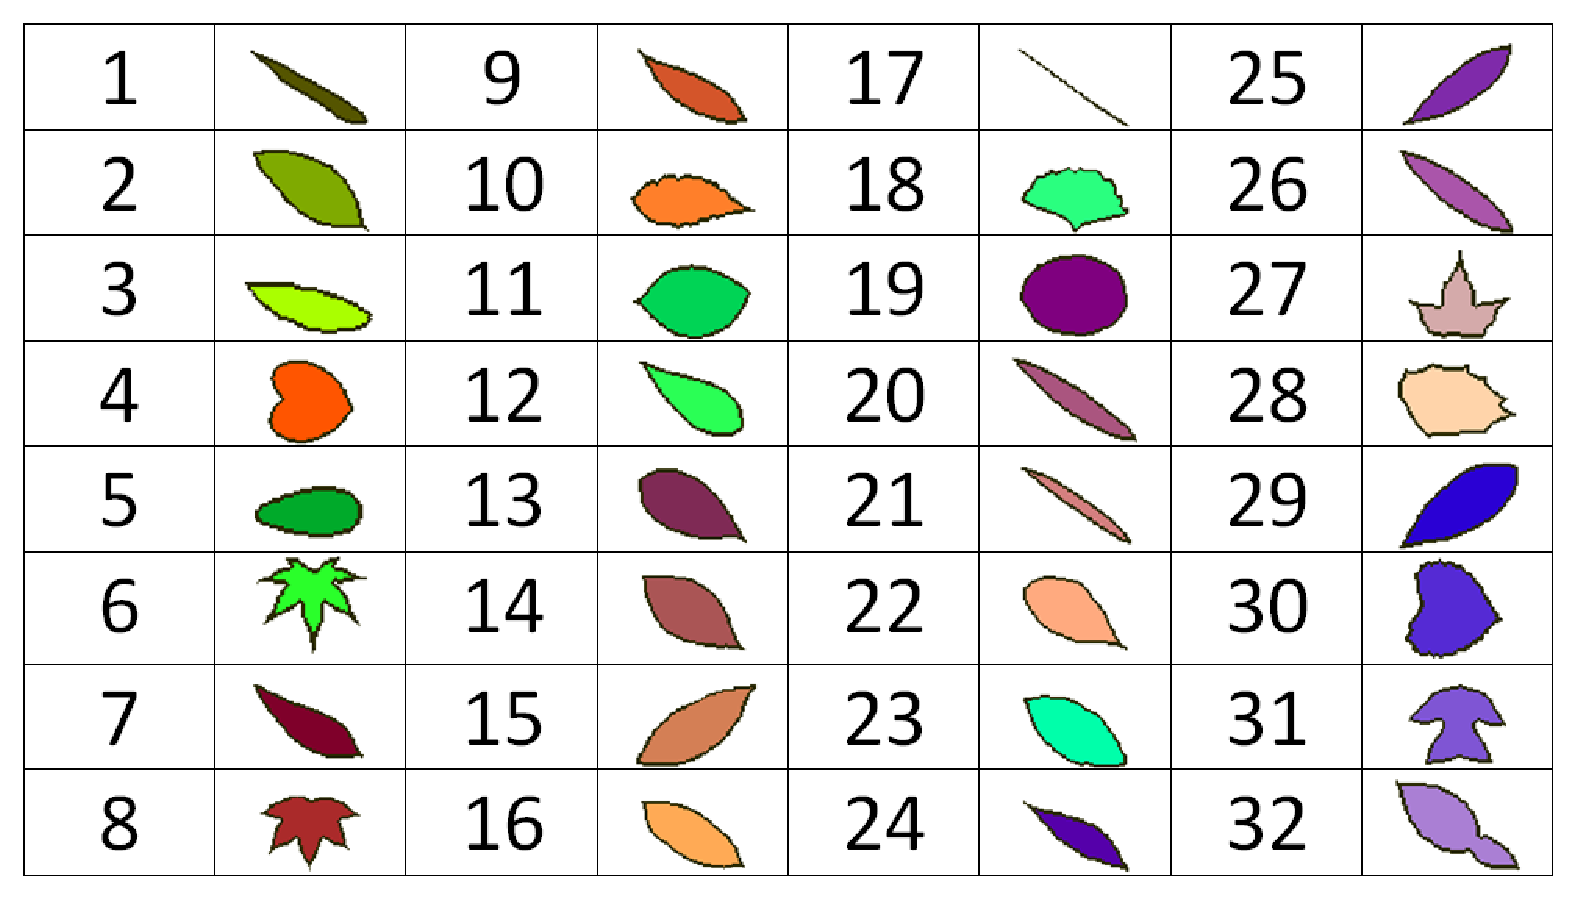
\includegraphics[width=0.5\textwidth]{fig5.eps}
\caption{\label{fig:bases}Samples of Flavia leaf data set.}
\end{figure}

